% Options for packages loaded elsewhere
\PassOptionsToPackage{unicode}{hyperref}
\PassOptionsToPackage{hyphens}{url}
\PassOptionsToPackage{dvipsnames,svgnames,x11names}{xcolor}
%
\documentclass[
]{article}

\usepackage{amsmath,amssymb}
\usepackage{lmodern}
\usepackage{iftex}
\ifPDFTeX
  \usepackage[T1]{fontenc}
  \usepackage[utf8]{inputenc}
  \usepackage{textcomp} % provide euro and other symbols
\else % if luatex or xetex
  \usepackage{unicode-math}
  \defaultfontfeatures{Scale=MatchLowercase}
  \defaultfontfeatures[\rmfamily]{Ligatures=TeX,Scale=1}
\fi
% Use upquote if available, for straight quotes in verbatim environments
\IfFileExists{upquote.sty}{\usepackage{upquote}}{}
\IfFileExists{microtype.sty}{% use microtype if available
  \usepackage[]{microtype}
  \UseMicrotypeSet[protrusion]{basicmath} % disable protrusion for tt fonts
}{}
\makeatletter
\@ifundefined{KOMAClassName}{% if non-KOMA class
  \IfFileExists{parskip.sty}{%
    \usepackage{parskip}
  }{% else
    \setlength{\parindent}{0pt}
    \setlength{\parskip}{6pt plus 2pt minus 1pt}}
}{% if KOMA class
  \KOMAoptions{parskip=half}}
\makeatother
\usepackage{xcolor}
\setlength{\emergencystretch}{3em} % prevent overfull lines
\setcounter{secnumdepth}{-\maxdimen} % remove section numbering
% Make \paragraph and \subparagraph free-standing
\ifx\paragraph\undefined\else
  \let\oldparagraph\paragraph
  \renewcommand{\paragraph}[1]{\oldparagraph{#1}\mbox{}}
\fi
\ifx\subparagraph\undefined\else
  \let\oldsubparagraph\subparagraph
  \renewcommand{\subparagraph}[1]{\oldsubparagraph{#1}\mbox{}}
\fi

\usepackage{color}
\usepackage{fancyvrb}
\newcommand{\VerbBar}{|}
\newcommand{\VERB}{\Verb[commandchars=\\\{\}]}
\DefineVerbatimEnvironment{Highlighting}{Verbatim}{commandchars=\\\{\}}
% Add ',fontsize=\small' for more characters per line
\usepackage{framed}
\definecolor{shadecolor}{RGB}{241,243,245}
\newenvironment{Shaded}{\begin{snugshade}}{\end{snugshade}}
\newcommand{\AlertTok}[1]{\textcolor[rgb]{0.68,0.00,0.00}{#1}}
\newcommand{\AnnotationTok}[1]{\textcolor[rgb]{0.37,0.37,0.37}{#1}}
\newcommand{\AttributeTok}[1]{\textcolor[rgb]{0.40,0.45,0.13}{#1}}
\newcommand{\BaseNTok}[1]{\textcolor[rgb]{0.68,0.00,0.00}{#1}}
\newcommand{\BuiltInTok}[1]{\textcolor[rgb]{0.00,0.23,0.31}{#1}}
\newcommand{\CharTok}[1]{\textcolor[rgb]{0.13,0.47,0.30}{#1}}
\newcommand{\CommentTok}[1]{\textcolor[rgb]{0.37,0.37,0.37}{#1}}
\newcommand{\CommentVarTok}[1]{\textcolor[rgb]{0.37,0.37,0.37}{\textit{#1}}}
\newcommand{\ConstantTok}[1]{\textcolor[rgb]{0.56,0.35,0.01}{#1}}
\newcommand{\ControlFlowTok}[1]{\textcolor[rgb]{0.00,0.23,0.31}{#1}}
\newcommand{\DataTypeTok}[1]{\textcolor[rgb]{0.68,0.00,0.00}{#1}}
\newcommand{\DecValTok}[1]{\textcolor[rgb]{0.68,0.00,0.00}{#1}}
\newcommand{\DocumentationTok}[1]{\textcolor[rgb]{0.37,0.37,0.37}{\textit{#1}}}
\newcommand{\ErrorTok}[1]{\textcolor[rgb]{0.68,0.00,0.00}{#1}}
\newcommand{\ExtensionTok}[1]{\textcolor[rgb]{0.00,0.23,0.31}{#1}}
\newcommand{\FloatTok}[1]{\textcolor[rgb]{0.68,0.00,0.00}{#1}}
\newcommand{\FunctionTok}[1]{\textcolor[rgb]{0.28,0.35,0.67}{#1}}
\newcommand{\ImportTok}[1]{\textcolor[rgb]{0.00,0.46,0.62}{#1}}
\newcommand{\InformationTok}[1]{\textcolor[rgb]{0.37,0.37,0.37}{#1}}
\newcommand{\KeywordTok}[1]{\textcolor[rgb]{0.00,0.23,0.31}{#1}}
\newcommand{\NormalTok}[1]{\textcolor[rgb]{0.00,0.23,0.31}{#1}}
\newcommand{\OperatorTok}[1]{\textcolor[rgb]{0.37,0.37,0.37}{#1}}
\newcommand{\OtherTok}[1]{\textcolor[rgb]{0.00,0.23,0.31}{#1}}
\newcommand{\PreprocessorTok}[1]{\textcolor[rgb]{0.68,0.00,0.00}{#1}}
\newcommand{\RegionMarkerTok}[1]{\textcolor[rgb]{0.00,0.23,0.31}{#1}}
\newcommand{\SpecialCharTok}[1]{\textcolor[rgb]{0.37,0.37,0.37}{#1}}
\newcommand{\SpecialStringTok}[1]{\textcolor[rgb]{0.13,0.47,0.30}{#1}}
\newcommand{\StringTok}[1]{\textcolor[rgb]{0.13,0.47,0.30}{#1}}
\newcommand{\VariableTok}[1]{\textcolor[rgb]{0.07,0.07,0.07}{#1}}
\newcommand{\VerbatimStringTok}[1]{\textcolor[rgb]{0.13,0.47,0.30}{#1}}
\newcommand{\WarningTok}[1]{\textcolor[rgb]{0.37,0.37,0.37}{\textit{#1}}}

\providecommand{\tightlist}{%
  \setlength{\itemsep}{0pt}\setlength{\parskip}{0pt}}\usepackage{longtable,booktabs,array}
\usepackage{calc} % for calculating minipage widths
% Correct order of tables after \paragraph or \subparagraph
\usepackage{etoolbox}
\makeatletter
\patchcmd\longtable{\par}{\if@noskipsec\mbox{}\fi\par}{}{}
\makeatother
% Allow footnotes in longtable head/foot
\IfFileExists{footnotehyper.sty}{\usepackage{footnotehyper}}{\usepackage{footnote}}
\makesavenoteenv{longtable}
\usepackage{graphicx}
\makeatletter
\def\maxwidth{\ifdim\Gin@nat@width>\linewidth\linewidth\else\Gin@nat@width\fi}
\def\maxheight{\ifdim\Gin@nat@height>\textheight\textheight\else\Gin@nat@height\fi}
\makeatother
% Scale images if necessary, so that they will not overflow the page
% margins by default, and it is still possible to overwrite the defaults
% using explicit options in \includegraphics[width, height, ...]{}
\setkeys{Gin}{width=\maxwidth,height=\maxheight,keepaspectratio}
% Set default figure placement to htbp
\makeatletter
\def\fps@figure{htbp}
\makeatother

\usepackage{booktabs}
\usepackage{longtable}
\usepackage{array}
\usepackage{multirow}
\usepackage{wrapfig}
\usepackage{float}
\usepackage{colortbl}
\usepackage{pdflscape}
\usepackage{tabu}
\usepackage{threeparttable}
\usepackage{threeparttablex}
\usepackage[normalem]{ulem}
\usepackage{makecell}
\usepackage{xcolor}
\usepackage{amsmath}
\usepackage{caption}
\makeatletter
\makeatother
\makeatletter
\makeatother
\makeatletter
\@ifpackageloaded{caption}{}{\usepackage{caption}}
\AtBeginDocument{%
\ifdefined\contentsname
  \renewcommand*\contentsname{Table of contents}
\else
  \newcommand\contentsname{Table of contents}
\fi
\ifdefined\listfigurename
  \renewcommand*\listfigurename{List of Figures}
\else
  \newcommand\listfigurename{List of Figures}
\fi
\ifdefined\listtablename
  \renewcommand*\listtablename{List of Tables}
\else
  \newcommand\listtablename{List of Tables}
\fi
\ifdefined\figurename
  \renewcommand*\figurename{Figure}
\else
  \newcommand\figurename{Figure}
\fi
\ifdefined\tablename
  \renewcommand*\tablename{Table}
\else
  \newcommand\tablename{Table}
\fi
}
\@ifpackageloaded{float}{}{\usepackage{float}}
\floatstyle{ruled}
\@ifundefined{c@chapter}{\newfloat{codelisting}{h}{lop}}{\newfloat{codelisting}{h}{lop}[chapter]}
\floatname{codelisting}{Listing}
\newcommand*\listoflistings{\listof{codelisting}{List of Listings}}
\makeatother
\makeatletter
\@ifpackageloaded{caption}{}{\usepackage{caption}}
\@ifpackageloaded{subcaption}{}{\usepackage{subcaption}}
\makeatother
\makeatletter
\@ifpackageloaded{tcolorbox}{}{\usepackage[many]{tcolorbox}}
\makeatother
\makeatletter
\@ifundefined{shadecolor}{\definecolor{shadecolor}{rgb}{.97, .97, .97}}
\makeatother
\makeatletter
\makeatother
\ifLuaTeX
  \usepackage{selnolig}  % disable illegal ligatures
\fi
\IfFileExists{bookmark.sty}{\usepackage{bookmark}}{\usepackage{hyperref}}
\IfFileExists{xurl.sty}{\usepackage{xurl}}{} % add URL line breaks if available
\urlstyle{same} % disable monospaced font for URLs
\hypersetup{
  pdftitle={test\_doc},
  pdfauthor={Janick Weberpals, RPh, PhD},
  colorlinks=true,
  linkcolor={blue},
  filecolor={Maroon},
  citecolor={Blue},
  urlcolor={Blue},
  pdfcreator={LaTeX via pandoc}}

\title{test\_doc}
\author{Janick Weberpals, RPh, PhD}
\date{4/12/23}

\begin{document}
\maketitle
\ifdefined\Shaded\renewenvironment{Shaded}{\begin{tcolorbox}[sharp corners, borderline west={3pt}{0pt}{shadecolor}, boxrule=0pt, interior hidden, breakable, enhanced, frame hidden]}{\end{tcolorbox}}\fi

\hypertarget{quarto}{%
\subsection{Quarto}\label{quarto}}

Quarto enables you to weave together content and executable code into a
finished document. To learn more about Quarto see
\url{https://quarto.org}.

\hypertarget{running-code}{%
\subsection{Running Code}\label{running-code}}

When you click the \textbf{Render} button a document will be generated
that includes both content and the output of embedded code. You can
embed code like this:

\begin{Shaded}
\begin{Highlighting}[]
\FunctionTok{library}\NormalTok{(dplyr)}
\end{Highlighting}
\end{Shaded}

\begin{verbatim}

Attaching package: 'dplyr'
\end{verbatim}

\begin{verbatim}
The following objects are masked from 'package:stats':

    filter, lag
\end{verbatim}

\begin{verbatim}
The following objects are masked from 'package:base':

    intersect, setdiff, setequal, union
\end{verbatim}

\begin{Shaded}
\begin{Highlighting}[]
\FunctionTok{library}\NormalTok{(gt)}
\FunctionTok{library}\NormalTok{(tableone)}
\FunctionTok{library}\NormalTok{(kableExtra)}
\end{Highlighting}
\end{Shaded}

\begin{verbatim}

Attaching package: 'kableExtra'
\end{verbatim}

\begin{verbatim}
The following object is masked from 'package:dplyr':

    group_rows
\end{verbatim}

\begin{Shaded}
\begin{Highlighting}[]
\NormalTok{devtools}\SpecialCharTok{::}\FunctionTok{load\_all}\NormalTok{()}
\end{Highlighting}
\end{Shaded}

\begin{verbatim}
i Loading toolbox
\end{verbatim}

\begin{verbatim}
Registered S3 method overwritten by 'webshot2':
  method        from   
  print.webshot webshot
\end{verbatim}

\newpage

\hypertarget{format_table}{%
\section{\texorpdfstring{\texttt{format\_table}}{format\_table}}\label{format_table}}

\hypertarget{normal-data}{%
\subsection{Normal data}\label{normal-data}}

\begin{Shaded}
\begin{Highlighting}[]
\NormalTok{data }\OtherTok{\textless{}{-}}\NormalTok{ dplyr}\SpecialCharTok{::}\FunctionTok{sample\_n}\NormalTok{(iris, }\DecValTok{10}\NormalTok{)}

\FunctionTok{format\_table}\NormalTok{(}
  \AttributeTok{data =}\NormalTok{ data,}
  \AttributeTok{font\_size =} \DecValTok{20}\NormalTok{,}
  \AttributeTok{caption =} \StringTok{"Normal data table"}
\NormalTok{  )}
\end{Highlighting}
\end{Shaded}

\begin{table}

\caption{\label{tbl-format_normal}\textbf{?(caption)}}\begin{minipage}[t]{\linewidth}
\subcaption{\label{tbl-format_normal-1}}

{\centering 

\begingroup\fontsize{20}{22}\selectfont

}

\end{minipage}%
\newline
\begin{minipage}[t]{\linewidth}
\subcaption{\label{tbl-format_normal-2}Normal data table}

{\centering 

\begin{longtable}[t]{lllll}
\\
\toprule
\textbf{Sepal.Length} & \textbf{Sepal.Width} & \textbf{Petal.Length} & \textbf{Petal.Width} & \textbf{Species}\\
\midrule
\endfirsthead
\caption[]{Normal data table \textit{(continued)}}\\
\toprule
\textbf{Sepal.Length} & \textbf{Sepal.Width} & \textbf{Petal.Length} & \textbf{Petal.Width} & \textbf{Species}\\
\midrule
\endhead

\endfoot
\bottomrule
\endlastfoot
6.9 & 3.2 & 5.7 & 2.3 & virginica\\
6.4 & 2.8 & 5.6 & 2.2 & virginica\\
6.0 & 2.7 & 5.1 & 1.6 & versicolor\\
5.8 & 2.7 & 5.1 & 1.9 & virginica\\
5.0 & 2.0 & 3.5 & 1.0 & versicolor\\
\addlinespace
6.1 & 3.0 & 4.6 & 1.4 & versicolor\\
5.4 & 3.4 & 1.7 & 0.2 & setosa\\
5.1 & 3.4 & 1.5 & 0.2 & setosa\\
4.7 & 3.2 & 1.3 & 0.2 & setosa\\
5.6 & 3.0 & 4.1 & 1.3 & versicolor\\*
\end{longtable}
\endgroup{}

}

\end{minipage}%

\end{table}

\hypertarget{table-1-with-format_table}{%
\subsection{\texorpdfstring{Table 1 with
\texttt{format\_table}}{Table 1 with format\_table}}\label{table-1-with-format_table}}

\begin{Shaded}
\begin{Highlighting}[]
\NormalTok{tbl1 }\OtherTok{\textless{}{-}}\NormalTok{ tableone}\SpecialCharTok{::}\FunctionTok{CreateTableOne}\NormalTok{(}
  \AttributeTok{data =}\NormalTok{ iris}
\NormalTok{  )}

\FunctionTok{format\_table}\NormalTok{(}
  \AttributeTok{data =}\NormalTok{ tbl1,}
  \AttributeTok{font\_size =} \DecValTok{20}\NormalTok{,}
  \AttributeTok{caption =} \StringTok{"Table 1 table"}
\NormalTok{  )}
\end{Highlighting}
\end{Shaded}

\begin{table}

\caption{\label{tbl-tbl1}\textbf{?(caption)}}\begin{minipage}[t]{\linewidth}
\subcaption{\label{tbl-tbl1-1}}

{\centering 

\begingroup\fontsize{20}{22}\selectfont

}

\end{minipage}%
\newline
\begin{minipage}[t]{\linewidth}
\subcaption{\label{tbl-tbl1-2}Table 1 table}

{\centering 

\begin{longtable}[t]{ll}
\\
\toprule
\textbf{Variable} & \textbf{Overall}\\
\midrule
\endfirsthead
\caption[]{Table 1 table \textit{(continued)}}\\
\toprule
\textbf{Variable} & \textbf{Overall}\\
\midrule
\endhead

\endfoot
\bottomrule
\endlastfoot
n & 150\\
Sepal.Length (mean (SD)) & 5.84 (0.83)\\
Sepal.Width (mean (SD)) & 3.06 (0.44)\\
Petal.Length (mean (SD)) & 3.76 (1.77)\\
Petal.Width (mean (SD)) & 1.20 (0.76)\\
\addlinespace
Species (\%) & \\
\hspace{1em}setosa & 50 (33.3)\\
\hspace{1em}versicolor & 50 (33.3)\\
\hspace{1em}virginica & 50 (33.3)\\*
\end{longtable}
\endgroup{}

}

\end{minipage}%

\end{table}

\hypertarget{long-table}{%
\subsection{Long table}\label{long-table}}

\begin{Shaded}
\begin{Highlighting}[]
\FunctionTok{format\_table}\NormalTok{(}
  \AttributeTok{data =}\NormalTok{ iris,}
  \AttributeTok{caption =} \StringTok{"Long table"}
\NormalTok{  )}
\end{Highlighting}
\end{Shaded}

\begingroup\fontsize{15}{17}\selectfont

\begin{longtable}[t]{lllll}
\caption{Long table}\\
\toprule
\textbf{Sepal.Length} & \textbf{Sepal.Width} & \textbf{Petal.Length} & \textbf{Petal.Width} & \textbf{Species}\\
\midrule
\endfirsthead
\caption[]{Long table \textit{(continued)}}\\
\toprule
\textbf{Sepal.Length} & \textbf{Sepal.Width} & \textbf{Petal.Length} & \textbf{Petal.Width} & \textbf{Species}\\
\midrule
\endhead

\endfoot
\bottomrule
\endlastfoot
5.1 & 3.5 & 1.4 & 0.2 & setosa\\
4.9 & 3.0 & 1.4 & 0.2 & setosa\\
4.7 & 3.2 & 1.3 & 0.2 & setosa\\
4.6 & 3.1 & 1.5 & 0.2 & setosa\\
5.0 & 3.6 & 1.4 & 0.2 & setosa\\
\addlinespace
5.4 & 3.9 & 1.7 & 0.4 & setosa\\
4.6 & 3.4 & 1.4 & 0.3 & setosa\\
5.0 & 3.4 & 1.5 & 0.2 & setosa\\
4.4 & 2.9 & 1.4 & 0.2 & setosa\\
4.9 & 3.1 & 1.5 & 0.1 & setosa\\
\addlinespace
5.4 & 3.7 & 1.5 & 0.2 & setosa\\
4.8 & 3.4 & 1.6 & 0.2 & setosa\\
4.8 & 3.0 & 1.4 & 0.1 & setosa\\
4.3 & 3.0 & 1.1 & 0.1 & setosa\\
5.8 & 4.0 & 1.2 & 0.2 & setosa\\
\addlinespace
5.7 & 4.4 & 1.5 & 0.4 & setosa\\
5.4 & 3.9 & 1.3 & 0.4 & setosa\\
5.1 & 3.5 & 1.4 & 0.3 & setosa\\
5.7 & 3.8 & 1.7 & 0.3 & setosa\\
5.1 & 3.8 & 1.5 & 0.3 & setosa\\
\addlinespace
5.4 & 3.4 & 1.7 & 0.2 & setosa\\
5.1 & 3.7 & 1.5 & 0.4 & setosa\\
4.6 & 3.6 & 1.0 & 0.2 & setosa\\
5.1 & 3.3 & 1.7 & 0.5 & setosa\\
4.8 & 3.4 & 1.9 & 0.2 & setosa\\
\addlinespace
5.0 & 3.0 & 1.6 & 0.2 & setosa\\
5.0 & 3.4 & 1.6 & 0.4 & setosa\\
5.2 & 3.5 & 1.5 & 0.2 & setosa\\
5.2 & 3.4 & 1.4 & 0.2 & setosa\\
4.7 & 3.2 & 1.6 & 0.2 & setosa\\
\addlinespace
4.8 & 3.1 & 1.6 & 0.2 & setosa\\
5.4 & 3.4 & 1.5 & 0.4 & setosa\\
5.2 & 4.1 & 1.5 & 0.1 & setosa\\
5.5 & 4.2 & 1.4 & 0.2 & setosa\\
4.9 & 3.1 & 1.5 & 0.2 & setosa\\
\addlinespace
5.0 & 3.2 & 1.2 & 0.2 & setosa\\
5.5 & 3.5 & 1.3 & 0.2 & setosa\\
4.9 & 3.6 & 1.4 & 0.1 & setosa\\
4.4 & 3.0 & 1.3 & 0.2 & setosa\\
5.1 & 3.4 & 1.5 & 0.2 & setosa\\
\addlinespace
5.0 & 3.5 & 1.3 & 0.3 & setosa\\
4.5 & 2.3 & 1.3 & 0.3 & setosa\\
4.4 & 3.2 & 1.3 & 0.2 & setosa\\
5.0 & 3.5 & 1.6 & 0.6 & setosa\\
5.1 & 3.8 & 1.9 & 0.4 & setosa\\
\addlinespace
4.8 & 3.0 & 1.4 & 0.3 & setosa\\
5.1 & 3.8 & 1.6 & 0.2 & setosa\\
4.6 & 3.2 & 1.4 & 0.2 & setosa\\
5.3 & 3.7 & 1.5 & 0.2 & setosa\\
5.0 & 3.3 & 1.4 & 0.2 & setosa\\
\addlinespace
7.0 & 3.2 & 4.7 & 1.4 & versicolor\\
6.4 & 3.2 & 4.5 & 1.5 & versicolor\\
6.9 & 3.1 & 4.9 & 1.5 & versicolor\\
5.5 & 2.3 & 4.0 & 1.3 & versicolor\\
6.5 & 2.8 & 4.6 & 1.5 & versicolor\\
\addlinespace
5.7 & 2.8 & 4.5 & 1.3 & versicolor\\
6.3 & 3.3 & 4.7 & 1.6 & versicolor\\
4.9 & 2.4 & 3.3 & 1.0 & versicolor\\
6.6 & 2.9 & 4.6 & 1.3 & versicolor\\
5.2 & 2.7 & 3.9 & 1.4 & versicolor\\
\addlinespace
5.0 & 2.0 & 3.5 & 1.0 & versicolor\\
5.9 & 3.0 & 4.2 & 1.5 & versicolor\\
6.0 & 2.2 & 4.0 & 1.0 & versicolor\\
6.1 & 2.9 & 4.7 & 1.4 & versicolor\\
5.6 & 2.9 & 3.6 & 1.3 & versicolor\\
\addlinespace
6.7 & 3.1 & 4.4 & 1.4 & versicolor\\
5.6 & 3.0 & 4.5 & 1.5 & versicolor\\
5.8 & 2.7 & 4.1 & 1.0 & versicolor\\
6.2 & 2.2 & 4.5 & 1.5 & versicolor\\
5.6 & 2.5 & 3.9 & 1.1 & versicolor\\
\addlinespace
5.9 & 3.2 & 4.8 & 1.8 & versicolor\\
6.1 & 2.8 & 4.0 & 1.3 & versicolor\\
6.3 & 2.5 & 4.9 & 1.5 & versicolor\\
6.1 & 2.8 & 4.7 & 1.2 & versicolor\\
6.4 & 2.9 & 4.3 & 1.3 & versicolor\\
\addlinespace
6.6 & 3.0 & 4.4 & 1.4 & versicolor\\
6.8 & 2.8 & 4.8 & 1.4 & versicolor\\
6.7 & 3.0 & 5.0 & 1.7 & versicolor\\
6.0 & 2.9 & 4.5 & 1.5 & versicolor\\
5.7 & 2.6 & 3.5 & 1.0 & versicolor\\
\addlinespace
5.5 & 2.4 & 3.8 & 1.1 & versicolor\\
5.5 & 2.4 & 3.7 & 1.0 & versicolor\\
5.8 & 2.7 & 3.9 & 1.2 & versicolor\\
6.0 & 2.7 & 5.1 & 1.6 & versicolor\\
5.4 & 3.0 & 4.5 & 1.5 & versicolor\\
\addlinespace
6.0 & 3.4 & 4.5 & 1.6 & versicolor\\
6.7 & 3.1 & 4.7 & 1.5 & versicolor\\
6.3 & 2.3 & 4.4 & 1.3 & versicolor\\
5.6 & 3.0 & 4.1 & 1.3 & versicolor\\
5.5 & 2.5 & 4.0 & 1.3 & versicolor\\
\addlinespace
5.5 & 2.6 & 4.4 & 1.2 & versicolor\\
6.1 & 3.0 & 4.6 & 1.4 & versicolor\\
5.8 & 2.6 & 4.0 & 1.2 & versicolor\\
5.0 & 2.3 & 3.3 & 1.0 & versicolor\\
5.6 & 2.7 & 4.2 & 1.3 & versicolor\\
\addlinespace
5.7 & 3.0 & 4.2 & 1.2 & versicolor\\
5.7 & 2.9 & 4.2 & 1.3 & versicolor\\
6.2 & 2.9 & 4.3 & 1.3 & versicolor\\
5.1 & 2.5 & 3.0 & 1.1 & versicolor\\
5.7 & 2.8 & 4.1 & 1.3 & versicolor\\
\addlinespace
6.3 & 3.3 & 6.0 & 2.5 & virginica\\
5.8 & 2.7 & 5.1 & 1.9 & \vphantom{1} virginica\\
7.1 & 3.0 & 5.9 & 2.1 & virginica\\
6.3 & 2.9 & 5.6 & 1.8 & virginica\\
6.5 & 3.0 & 5.8 & 2.2 & virginica\\
\addlinespace
7.6 & 3.0 & 6.6 & 2.1 & virginica\\
4.9 & 2.5 & 4.5 & 1.7 & virginica\\
7.3 & 2.9 & 6.3 & 1.8 & virginica\\
6.7 & 2.5 & 5.8 & 1.8 & virginica\\
7.2 & 3.6 & 6.1 & 2.5 & virginica\\
\addlinespace
6.5 & 3.2 & 5.1 & 2.0 & virginica\\
6.4 & 2.7 & 5.3 & 1.9 & virginica\\
6.8 & 3.0 & 5.5 & 2.1 & virginica\\
5.7 & 2.5 & 5.0 & 2.0 & virginica\\
5.8 & 2.8 & 5.1 & 2.4 & virginica\\
\addlinespace
6.4 & 3.2 & 5.3 & 2.3 & virginica\\
6.5 & 3.0 & 5.5 & 1.8 & virginica\\
7.7 & 3.8 & 6.7 & 2.2 & virginica\\
7.7 & 2.6 & 6.9 & 2.3 & virginica\\
6.0 & 2.2 & 5.0 & 1.5 & virginica\\
\addlinespace
6.9 & 3.2 & 5.7 & 2.3 & virginica\\
5.6 & 2.8 & 4.9 & 2.0 & virginica\\
7.7 & 2.8 & 6.7 & 2.0 & virginica\\
6.3 & 2.7 & 4.9 & 1.8 & virginica\\
6.7 & 3.3 & 5.7 & 2.1 & virginica\\
\addlinespace
7.2 & 3.2 & 6.0 & 1.8 & virginica\\
6.2 & 2.8 & 4.8 & 1.8 & virginica\\
6.1 & 3.0 & 4.9 & 1.8 & virginica\\
6.4 & 2.8 & 5.6 & 2.1 & virginica\\
7.2 & 3.0 & 5.8 & 1.6 & virginica\\
\addlinespace
7.4 & 2.8 & 6.1 & 1.9 & virginica\\
7.9 & 3.8 & 6.4 & 2.0 & virginica\\
6.4 & 2.8 & 5.6 & 2.2 & virginica\\
6.3 & 2.8 & 5.1 & 1.5 & virginica\\
6.1 & 2.6 & 5.6 & 1.4 & virginica\\
\addlinespace
7.7 & 3.0 & 6.1 & 2.3 & virginica\\
6.3 & 3.4 & 5.6 & 2.4 & virginica\\
6.4 & 3.1 & 5.5 & 1.8 & virginica\\
6.0 & 3.0 & 4.8 & 1.8 & virginica\\
6.9 & 3.1 & 5.4 & 2.1 & virginica\\
\addlinespace
6.7 & 3.1 & 5.6 & 2.4 & virginica\\
6.9 & 3.1 & 5.1 & 2.3 & virginica\\
5.8 & 2.7 & 5.1 & 1.9 & virginica\\
6.8 & 3.2 & 5.9 & 2.3 & virginica\\
6.7 & 3.3 & 5.7 & 2.5 & virginica\\
\addlinespace
6.7 & 3.0 & 5.2 & 2.3 & virginica\\
6.3 & 2.5 & 5.0 & 1.9 & virginica\\
6.5 & 3.0 & 5.2 & 2.0 & virginica\\
6.2 & 3.4 & 5.4 & 2.3 & virginica\\
5.9 & 3.0 & 5.1 & 1.8 & virginica\\*
\end{longtable}
\endgroup{}

\hypertarget{standard-functions}{%
\section{Standard functions}\label{standard-functions}}

\hypertarget{kableextra-latex-test}{%
\subsection{kableExtra (latex test)}\label{kableextra-latex-test}}

\begin{Shaded}
\begin{Highlighting}[]
\NormalTok{data }\OtherTok{\textless{}{-}}\NormalTok{ dplyr}\SpecialCharTok{::}\FunctionTok{sample\_n}\NormalTok{(iris, }\DecValTok{80}\NormalTok{)}

\NormalTok{data }\SpecialCharTok{\%\textgreater{}\%} 
\NormalTok{  kableExtra}\SpecialCharTok{::} \FunctionTok{kbl}\NormalTok{(}
    \AttributeTok{booktabs =} \ConstantTok{TRUE}\NormalTok{,}
    \AttributeTok{longtable =} \ConstantTok{TRUE}\NormalTok{,}
    \AttributeTok{caption =} \StringTok{"Test table 3"}
\NormalTok{  ) }\SpecialCharTok{\%\textgreater{}\%} 
\NormalTok{  kableExtra}\SpecialCharTok{::}\FunctionTok{kable\_styling}\NormalTok{(}
    \AttributeTok{latex\_options =} \FunctionTok{c}\NormalTok{(}\StringTok{"repeat\_header"}\NormalTok{),}
    \AttributeTok{repeat\_header\_continued =} \StringTok{"}\SpecialCharTok{\textbackslash{}\textbackslash{}}\StringTok{textit\{(Continued on next page...)\}"}\NormalTok{,}
\NormalTok{    )}
\end{Highlighting}
\end{Shaded}

\begin{longtable}[t]{rrrrl}
\caption{Test table 3}\\
\toprule
Sepal.Length & Sepal.Width & Petal.Length & Petal.Width & Species\\
\midrule
\endfirsthead
\caption[]{Test table 3 \textit{(continued)}}\\
\toprule
Sepal.Length & Sepal.Width & Petal.Length & Petal.Width & Species\\
\midrule
\endhead
\midrule
\multicolumn{5}{r@{}}{\textit{(Continued on next page...)}}\
\endfoot
\bottomrule
\endlastfoot
6.4 & 2.7 & 5.3 & 1.9 & virginica\\
4.4 & 3.2 & 1.3 & 0.2 & setosa\\
4.9 & 2.5 & 4.5 & 1.7 & virginica\\
5.4 & 3.4 & 1.7 & 0.2 & setosa\\
6.2 & 2.9 & 4.3 & 1.3 & versicolor\\
\addlinespace
6.3 & 3.3 & 6.0 & 2.5 & virginica\\
5.1 & 3.4 & 1.5 & 0.2 & setosa\\
4.6 & 3.1 & 1.5 & 0.2 & setosa\\
5.6 & 3.0 & 4.1 & 1.3 & versicolor\\
6.4 & 3.2 & 4.5 & 1.5 & versicolor\\
\addlinespace
5.0 & 3.4 & 1.5 & 0.2 & setosa\\
5.0 & 2.3 & 3.3 & 1.0 & versicolor\\
6.1 & 2.8 & 4.0 & 1.3 & versicolor\\
5.0 & 3.3 & 1.4 & 0.2 & setosa\\
6.1 & 2.8 & 4.7 & 1.2 & versicolor\\
\addlinespace
6.2 & 2.2 & 4.5 & 1.5 & versicolor\\
5.6 & 3.0 & 4.5 & 1.5 & versicolor\\
6.7 & 3.1 & 4.4 & 1.4 & versicolor\\
6.8 & 3.0 & 5.5 & 2.1 & virginica\\
7.2 & 3.6 & 6.1 & 2.5 & virginica\\
\addlinespace
5.2 & 3.4 & 1.4 & 0.2 & setosa\\
5.4 & 3.9 & 1.7 & 0.4 & setosa\\
6.5 & 3.2 & 5.1 & 2.0 & virginica\\
6.4 & 2.8 & 5.6 & 2.2 & virginica\\
7.7 & 3.8 & 6.7 & 2.2 & virginica\\
\addlinespace
4.9 & 3.1 & 1.5 & 0.1 & setosa\\
5.7 & 2.6 & 3.5 & 1.0 & versicolor\\
5.8 & 2.8 & 5.1 & 2.4 & virginica\\
6.9 & 3.2 & 5.7 & 2.3 & virginica\\
5.8 & 2.7 & 3.9 & 1.2 & versicolor\\
\addlinespace
6.3 & 3.4 & 5.6 & 2.4 & virginica\\
6.0 & 2.2 & 4.0 & 1.0 & versicolor\\
6.0 & 2.7 & 5.1 & 1.6 & versicolor\\
5.1 & 3.7 & 1.5 & 0.4 & setosa\\
7.2 & 3.2 & 6.0 & 1.8 & virginica\\
\addlinespace
7.7 & 2.8 & 6.7 & 2.0 & virginica\\
6.6 & 3.0 & 4.4 & 1.4 & versicolor\\
4.4 & 3.0 & 1.3 & 0.2 & setosa\\
6.0 & 2.9 & 4.5 & 1.5 & versicolor\\
5.1 & 3.8 & 1.9 & 0.4 & setosa\\
\addlinespace
5.0 & 3.2 & 1.2 & 0.2 & setosa\\
5.7 & 2.8 & 4.1 & 1.3 & versicolor\\
5.5 & 2.3 & 4.0 & 1.3 & versicolor\\
7.1 & 3.0 & 5.9 & 2.1 & virginica\\
6.2 & 3.4 & 5.4 & 2.3 & virginica\\
\addlinespace
5.7 & 4.4 & 1.5 & 0.4 & setosa\\
4.8 & 3.1 & 1.6 & 0.2 & setosa\\
7.7 & 3.0 & 6.1 & 2.3 & virginica\\
6.8 & 3.2 & 5.9 & 2.3 & virginica\\
6.2 & 2.8 & 4.8 & 1.8 & virginica\\
\addlinespace
6.0 & 3.4 & 4.5 & 1.6 & versicolor\\
5.0 & 3.0 & 1.6 & 0.2 & setosa\\
6.5 & 2.8 & 4.6 & 1.5 & versicolor\\
5.7 & 2.9 & 4.2 & 1.3 & versicolor\\
4.8 & 3.0 & 1.4 & 0.3 & setosa\\
\addlinespace
4.7 & 3.2 & 1.3 & 0.2 & setosa\\
5.1 & 3.5 & 1.4 & 0.2 & setosa\\
5.9 & 3.2 & 4.8 & 1.8 & versicolor\\
6.0 & 3.0 & 4.8 & 1.8 & virginica\\
5.1 & 3.5 & 1.4 & 0.3 & setosa\\
\addlinespace
6.7 & 3.3 & 5.7 & 2.1 & virginica\\
7.3 & 2.9 & 6.3 & 1.8 & virginica\\
6.3 & 2.5 & 4.9 & 1.5 & versicolor\\
5.5 & 4.2 & 1.4 & 0.2 & setosa\\
6.9 & 3.1 & 5.1 & 2.3 & virginica\\
\addlinespace
4.4 & 2.9 & 1.4 & 0.2 & setosa\\
5.1 & 3.8 & 1.6 & 0.2 & setosa\\
6.7 & 3.1 & 5.6 & 2.4 & virginica\\
4.9 & 3.1 & 1.5 & 0.2 & setosa\\
5.1 & 3.8 & 1.5 & 0.3 & setosa\\
\addlinespace
5.4 & 3.7 & 1.5 & 0.2 & setosa\\
5.1 & 2.5 & 3.0 & 1.1 & versicolor\\
6.6 & 2.9 & 4.6 & 1.3 & versicolor\\
5.0 & 3.4 & 1.6 & 0.4 & setosa\\
6.5 & 3.0 & 5.2 & 2.0 & virginica\\
\addlinespace
6.1 & 2.6 & 5.6 & 1.4 & virginica\\
4.8 & 3.4 & 1.9 & 0.2 & setosa\\
5.5 & 2.4 & 3.8 & 1.1 & versicolor\\
7.4 & 2.8 & 6.1 & 1.9 & virginica\\
6.9 & 3.1 & 5.4 & 2.1 & virginica\\*
\end{longtable}

\& 2.1 \& virginica\textbackslash* \textbackslash end\{longtable\}

\hypertarget{gt}{%
\subsection{gt}\label{gt}}

\textbf{Table 4.} Table caption\ldots{}

\begin{longtable}{rrrrc}
\toprule
Sepal.Length & Sepal.Width & Petal.Length & Petal.Width & Species \\ 
\midrule
6.4 & 2.7 & 5.3 & 1.9 & virginica \\ 
4.4 & 3.2 & 1.3 & 0.2 & setosa \\ 
4.9 & 2.5 & 4.5 & 1.7 & virginica \\ 
5.4 & 3.4 & 1.7 & 0.2 & setosa \\ 
6.2 & 2.9 & 4.3 & 1.3 & versicolor \\ 
6.3 & 3.3 & 6.0 & 2.5 & virginica \\ 
5.1 & 3.4 & 1.5 & 0.2 & setosa \\ 
4.6 & 3.1 & 1.5 & 0.2 & setosa \\ 
5.6 & 3.0 & 4.1 & 1.3 & versicolor \\ 
6.4 & 3.2 & 4.5 & 1.5 & versicolor \\ 
5.0 & 3.4 & 1.5 & 0.2 & setosa \\ 
5.0 & 2.3 & 3.3 & 1.0 & versicolor \\ 
6.1 & 2.8 & 4.0 & 1.3 & versicolor \\ 
5.0 & 3.3 & 1.4 & 0.2 & setosa \\ 
6.1 & 2.8 & 4.7 & 1.2 & versicolor \\ 
6.2 & 2.2 & 4.5 & 1.5 & versicolor \\ 
5.6 & 3.0 & 4.5 & 1.5 & versicolor \\ 
6.7 & 3.1 & 4.4 & 1.4 & versicolor \\ 
6.8 & 3.0 & 5.5 & 2.1 & virginica \\ 
7.2 & 3.6 & 6.1 & 2.5 & virginica \\ 
5.2 & 3.4 & 1.4 & 0.2 & setosa \\ 
5.4 & 3.9 & 1.7 & 0.4 & setosa \\ 
6.5 & 3.2 & 5.1 & 2.0 & virginica \\ 
6.4 & 2.8 & 5.6 & 2.2 & virginica \\ 
7.7 & 3.8 & 6.7 & 2.2 & virginica \\ 
4.9 & 3.1 & 1.5 & 0.1 & setosa \\ 
5.7 & 2.6 & 3.5 & 1.0 & versicolor \\ 
5.8 & 2.8 & 5.1 & 2.4 & virginica \\ 
6.9 & 3.2 & 5.7 & 2.3 & virginica \\ 
5.8 & 2.7 & 3.9 & 1.2 & versicolor \\ 
6.3 & 3.4 & 5.6 & 2.4 & virginica \\ 
6.0 & 2.2 & 4.0 & 1.0 & versicolor \\ 
6.0 & 2.7 & 5.1 & 1.6 & versicolor \\ 
5.1 & 3.7 & 1.5 & 0.4 & setosa \\ 
7.2 & 3.2 & 6.0 & 1.8 & virginica \\ 
7.7 & 2.8 & 6.7 & 2.0 & virginica \\ 
6.6 & 3.0 & 4.4 & 1.4 & versicolor \\ 
4.4 & 3.0 & 1.3 & 0.2 & setosa \\ 
6.0 & 2.9 & 4.5 & 1.5 & versicolor \\ 
5.1 & 3.8 & 1.9 & 0.4 & setosa \\ 
5.0 & 3.2 & 1.2 & 0.2 & setosa \\ 
5.7 & 2.8 & 4.1 & 1.3 & versicolor \\ 
5.5 & 2.3 & 4.0 & 1.3 & versicolor \\ 
7.1 & 3.0 & 5.9 & 2.1 & virginica \\ 
6.2 & 3.4 & 5.4 & 2.3 & virginica \\ 
5.7 & 4.4 & 1.5 & 0.4 & setosa \\ 
4.8 & 3.1 & 1.6 & 0.2 & setosa \\ 
7.7 & 3.0 & 6.1 & 2.3 & virginica \\ 
6.8 & 3.2 & 5.9 & 2.3 & virginica \\ 
6.2 & 2.8 & 4.8 & 1.8 & virginica \\ 
6.0 & 3.4 & 4.5 & 1.6 & versicolor \\ 
5.0 & 3.0 & 1.6 & 0.2 & setosa \\ 
6.5 & 2.8 & 4.6 & 1.5 & versicolor \\ 
5.7 & 2.9 & 4.2 & 1.3 & versicolor \\ 
4.8 & 3.0 & 1.4 & 0.3 & setosa \\ 
4.7 & 3.2 & 1.3 & 0.2 & setosa \\ 
5.1 & 3.5 & 1.4 & 0.2 & setosa \\ 
5.9 & 3.2 & 4.8 & 1.8 & versicolor \\ 
6.0 & 3.0 & 4.8 & 1.8 & virginica \\ 
5.1 & 3.5 & 1.4 & 0.3 & setosa \\ 
6.7 & 3.3 & 5.7 & 2.1 & virginica \\ 
7.3 & 2.9 & 6.3 & 1.8 & virginica \\ 
6.3 & 2.5 & 4.9 & 1.5 & versicolor \\ 
5.5 & 4.2 & 1.4 & 0.2 & setosa \\ 
6.9 & 3.1 & 5.1 & 2.3 & virginica \\ 
4.4 & 2.9 & 1.4 & 0.2 & setosa \\ 
5.1 & 3.8 & 1.6 & 0.2 & setosa \\ 
6.7 & 3.1 & 5.6 & 2.4 & virginica \\ 
4.9 & 3.1 & 1.5 & 0.2 & setosa \\ 
5.1 & 3.8 & 1.5 & 0.3 & setosa \\ 
5.4 & 3.7 & 1.5 & 0.2 & setosa \\ 
5.1 & 2.5 & 3.0 & 1.1 & versicolor \\ 
6.6 & 2.9 & 4.6 & 1.3 & versicolor \\ 
5.0 & 3.4 & 1.6 & 0.4 & setosa \\ 
6.5 & 3.0 & 5.2 & 2.0 & virginica \\ 
6.1 & 2.6 & 5.6 & 1.4 & virginica \\ 
4.8 & 3.4 & 1.9 & 0.2 & setosa \\ 
5.5 & 2.4 & 3.8 & 1.1 & versicolor \\ 
7.4 & 2.8 & 6.1 & 1.9 & virginica \\ 
6.9 & 3.1 & 5.4 & 2.1 & virginica \\ 
\bottomrule
\end{longtable}

\hypertarget{format_gt-test}{%
\section{\texorpdfstring{\texttt{format\_gt}
test}{format\_gt test}}\label{format_gt-test}}

\begin{Shaded}
\begin{Highlighting}[]
\NormalTok{iris\_gt }\OtherTok{\textless{}{-}} \FunctionTok{head}\NormalTok{(iris) }\SpecialCharTok{\%\textgreater{}\%} 
\NormalTok{  gt}\SpecialCharTok{::}\FunctionTok{gt}\NormalTok{()}

\FunctionTok{format\_gt}\NormalTok{(}\AttributeTok{tbl\_gt =}\NormalTok{ iris\_gt, }\AttributeTok{zoom =} \DecValTok{1}\NormalTok{)}
\end{Highlighting}
\end{Shaded}

\begin{table}

\caption{\textbf{?(caption)}}\begin{minipage}[t]{\linewidth}

{\centering 

\raisebox{-\height}{

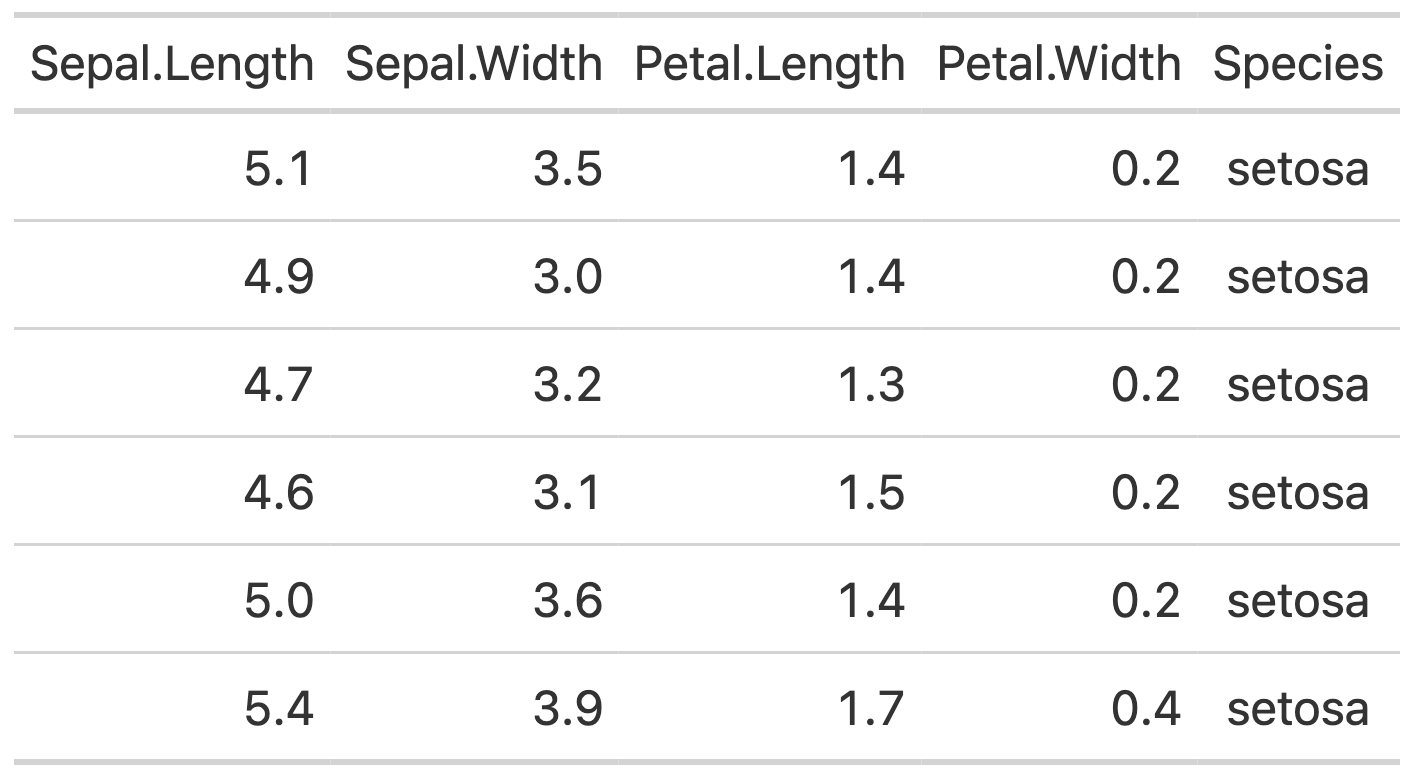
\includegraphics[width=1.57in,height=\textheight]{../gt_tables/iris_gt.png}

}

}

\end{minipage}%

\end{table}

\begin{Shaded}
\begin{Highlighting}[]
\NormalTok{iris\_gt }\OtherTok{\textless{}{-}} \FunctionTok{head}\NormalTok{(iris) }\SpecialCharTok{\%\textgreater{}\%} 
\NormalTok{  gt}\SpecialCharTok{::}\FunctionTok{gt}\NormalTok{()}

\FunctionTok{format\_gt}\NormalTok{(}\AttributeTok{tbl\_gt =}\NormalTok{ iris\_gt, }\AttributeTok{zoom =} \DecValTok{1}\NormalTok{)}
\end{Highlighting}
\end{Shaded}

\begin{table}

\caption{\textbf{?(caption)}}\begin{minipage}[t]{\linewidth}

{\centering 

\raisebox{-\height}{

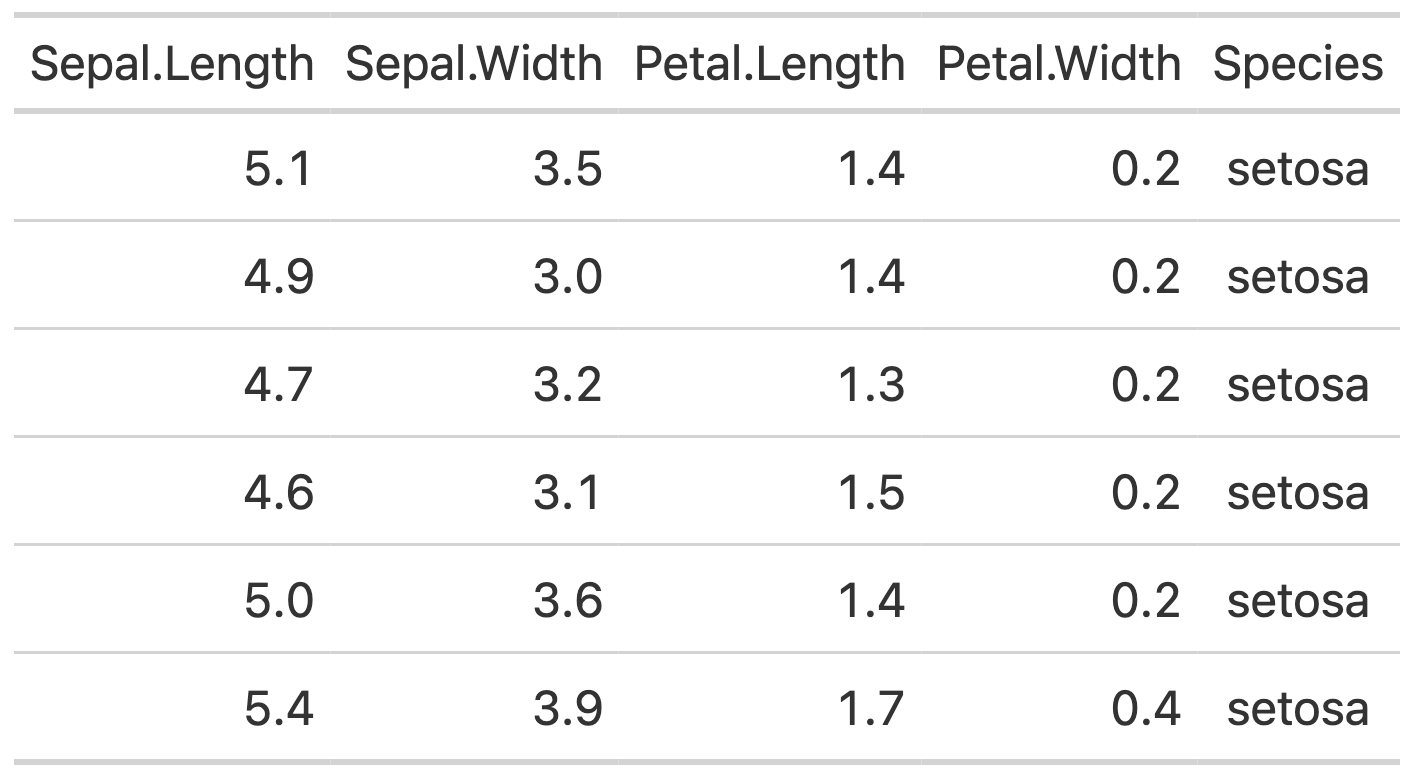
\includegraphics[width=1.57in,height=\textheight]{../gt_tables/iris_gt.png}

}

}

\end{minipage}%

\end{table}

\begin{Shaded}
\begin{Highlighting}[]
\NormalTok{iris\_gt }\OtherTok{\textless{}{-}} \FunctionTok{head}\NormalTok{(iris) }\SpecialCharTok{\%\textgreater{}\%} 
\NormalTok{  gt}\SpecialCharTok{::}\FunctionTok{gt}\NormalTok{()}

\FunctionTok{format\_gt}\NormalTok{(}\AttributeTok{tbl\_gt =}\NormalTok{ iris\_gt, }\AttributeTok{zoom =} \DecValTok{1}\NormalTok{, }\AttributeTok{dpi =} \DecValTok{500}\NormalTok{)}
\end{Highlighting}
\end{Shaded}

\begin{table}

\caption{\textbf{?(caption)}}\begin{minipage}[t]{\linewidth}

{\centering 

\raisebox{-\height}{

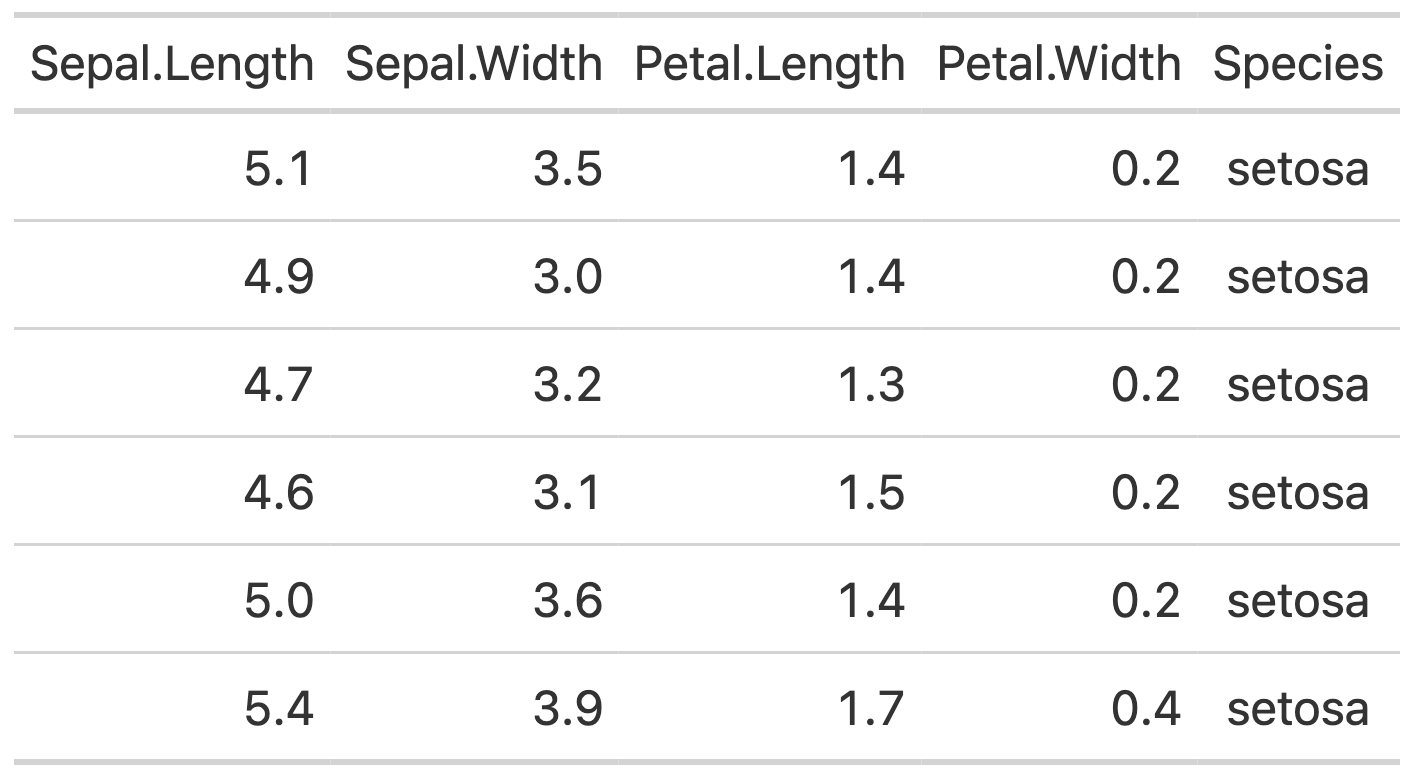
\includegraphics[width=0.94in,height=\textheight]{../gt_tables/iris_gt.png}

}

}

\end{minipage}%

\end{table}

\begin{Shaded}
\begin{Highlighting}[]
\NormalTok{gt}\SpecialCharTok{::}\FunctionTok{gtsave}\NormalTok{(}
  \AttributeTok{data =}\NormalTok{ iris\_gt,}
  \AttributeTok{filename =} \StringTok{"iris\_gt.docx"}\NormalTok{,}
  \AttributeTok{path =}\NormalTok{ here}\SpecialCharTok{::}\FunctionTok{here}\NormalTok{(}\StringTok{"gt\_tables"}\NormalTok{)}
\NormalTok{  )}
\end{Highlighting}
\end{Shaded}

\begin{table}

\caption{\textbf{?(caption)}}

\end{table}



\end{document}
